\documentclass[11pt, english]{article}

%% Math
\usepackage{amsmath}
\usepackage{dsfont}
\DeclareMathOperator{\Exists}{\exists}
\DeclareMathOperator{\Forall}{\forall}

%% Language and Encoding
\usepackage[T1]{fontenc}
\usepackage[english]{babel}
\usepackage[utf8]{inputenc}
\usepackage{varioref}
\usepackage{hyperref}
\usepackage[font={small,it}]{caption}

%% Title and Header
\usepackage{fancyhdr}
\makeatletter
\title{Named-Entity Recognition Project\\Documentation}
\let\Title\@title
\def\Subtitle{Natural Language Processing and the Web}
\author{Florian Schneider, Julian Betz}
\let\Author\@author
\date{\today}
\let\Date\@date
\renewcommand\@maketitle{\noindent\rule{\textwidth}{0.4pt}\par{\centering\LARGE\textbf{\@title}\par\Subtitle\par}\noindent\rule{\textwidth}{0.4pt}\vspace{3ex}\par\noindent\@author\hfill\@date\vspace{3ex}\par}
\makeatother
\fancypagestyle{mainmatter}{\fancyhf{}\renewcommand{\headrulewidth}{0.4pt}\lhead{\Author}\rhead{\textsc{NER Project Documentation}}\cfoot{\thepage}}

\setlength\parindent{1em}

%% Grafik
\usepackage{tikz}
\tikzset{>=latex}

\begin{document}
\maketitle

\pagestyle{mainmatter}

\section{Newly implemented classes}
The following classes were newly implemented in \url{de.unihamburg.informatik.nlp4web.tutorial.tut5}.

\subsection{\texttt{writer.NERWriter}}
An Analysis Engine that processes a CAS to generate the evaluation file and to calculate statistics for the \verb/NEIOBAnnotations/ generated earlier in the pipeline.
It finds all \verb/NEIOBAnnotations/ that have an attached prediction value and searches for the \verb/NEIOBAnnotation/ that has the corresponding gold standard value.
Each gold standard / prediction pair, along with the corresponding token, is printed to a text file that can be used as input for the evaluation scripts.

For each gold standard value, the number of predictions of each named-entity type is shown in the output.
As an aggregate result, the absolute and relative amounts of correct classification are given.
Furthermore, a table is generated that shows the number of classifications of a token as a named entity or non-named entity.
Finally, the absolute and relative amounts of correct classification of tokens that are named entities according to the gold standard are given.
(This number may be of interest as there are far more non-named entities than named entities in the data, according to the gold standard.)

\subsubsection{Configuration parameters}
The configuration parameter \verb/PARAM_FILENAME/ is the filename of the evaluation file to be generated.

The configuration parameter \verb/PARAM_NULL_TYPE/ determines which string is used for marking non-named entities in the input.
(Set to ``O'' in our case.)

If the configuration parameter \verb/PARAM_VERBOSE/ is set to \verb/true/, all incorrect predictions are printed out to the log before printing the statistics.

The configuration parameter \verb/PARAM_EXPECTED_ENTITY_TYPE_NUM/ is used for the initialization of data structures and only affects efficiency, but not functionality.

\subsection{\texttt{NEListExtractor}}
This class provides a functionallity to create a feature if the covered text of a token appears in a gazetteer. As shown in figure \ref{fig:NEListExtractor}, the \verb/NEListExtractor/ class implements the \verb/FeatureFunction/ interface. This is because this feature extractor works on the covered text of a token as mentioned before. Therefore, to use the \verb/NEListExtractor/ one has to do use it with the \verb/CoveredTextExtractor/ from the ClearTK Framework. An example can be seen in figure \ref{fig:NEListExtractorSample}.

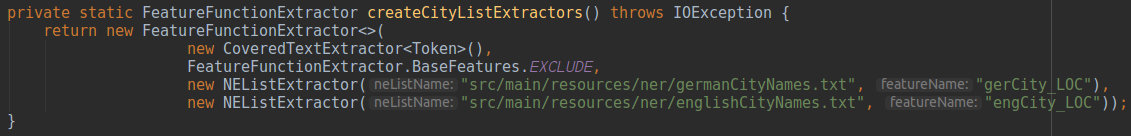
\includegraphics[width=\linewidth, keepaspectratio]{gfx/createNEListExtractor.png}
\captionof{figure}{Example on how to use NEListExtractors}
\label{fig:NEListExtractorSample}

Please note, that in the example two \verb/NEListExtractor/s are instantiated with two different gazetteers and feature names. The constructor of the \verb/NEListAnnotator/ requires two Strings, which represent the name (or path) to the list of Named Entities and the value of the feature that'll be created, respectivley (see \ref{fig:NEListExtractor}). The provided list of Named Entities that will be used by the \verb/NEListExtractor/ has to contain one single column. Each row contains one word, that represent the Named Entity. Please note, that it is not possible to use e.g. 'New York' as a single Named Entity since it contains a space. This restriction is due to the \verb/CoveredTextExtractor/ that only 'looks' at one Token at a time and the Segmenter which is used in the pipeline creates two Tokens in this case - namlely 'New' and 'York'. Theoretically this can be changed by using a better Segmenter or using a different \verb/TokenFeatureExtractor/ than the \verb/CoveredTextExtractor/, that takes multiple Tokens at a time in account.

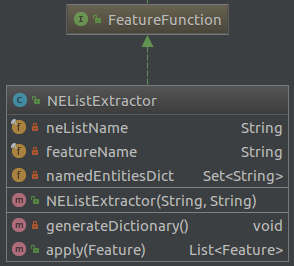
\includegraphics[scale=0.75]{gfx/NEListExtractor.png}
\captionof{figure}{Class diagram of the NEListExtractor}
\label{fig:NEListExtractor}

The functionallity of the \verb/NEListExtractor/ is implemented in the overridden \verb/apply()/ method. A graphical representation of this method can be seen in \ref{fig:NEListExtractorApply}. Whenn the \verb/apply()/ method gets called (indirectly from the \verb/NERAnnotator/) at first the list of Named Entities gets generated in the \verb/generateDicionary()/ method. This is simply done by reading the list file line by line and storing the Named Enity in a Hash Set for fast look up. Since this has to be done only once and not everytime the apply() method gets called, there is a check if the dict has already been initialized. Then a simple look up of the Tokens covered text in the dictionary is done. If it appears in the dictionary, a Feature for the Token that holds the neListName as Features name and featureValue as the Features value member variables gets created. Since the interface of the \verb/apply()/ method requires a list of Features as return type, the Feature gets added to a singleton list (i.e. an immuatable list that only contains one item). If the list of named entities does not contain the Tokens covered text an empty list will be returned.

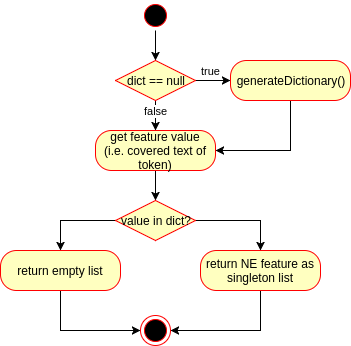
\includegraphics[scale=0.75]{gfx/apply.png}
\captionof{figure}{Activity diagram of the apply() method of NEListExtractor}
\label{fig:NEListExtractorApply}

\subsection{\texttt{FeatureExtractorFactory}}
\label{sec:FeatureExtractorFactory}
This class only serves as untility class to instantiate the different Feature Extractors that will be used during NER and helps to reduce code redundancy. The class diagram is shown in figure \ref{fig:FeatureExtractorFactory}The names of the methods represent exactly what the method does - no magic at all.

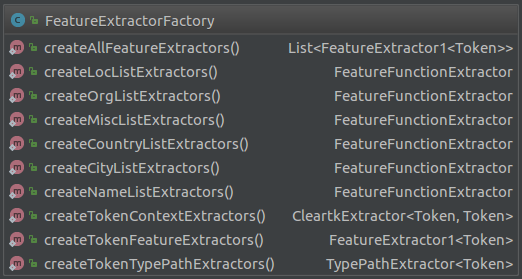
\includegraphics[scale=0.5]{gfx/FeatureExtractorFactory.png}
\captionof{figure}{Class diagram of the FeatureExtractorFactory}
\label{fig:FeatureExtractorFactory}

\subsection{\texttt{AblationTestRunner}}
\label{sec:AblationTestRunner}
This class implements the Runnable interface and holds the algorithm of one single run 'ablation test run'. %%TODO

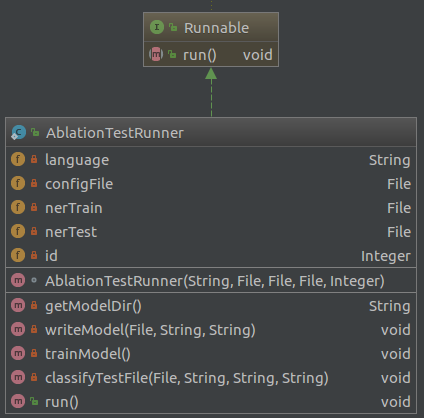
\includegraphics[scale=0.5]{gfx/AblationTestRunner.png}
\captionof{figure}{Class diagram of the AblationTestRunner}
\label{fig:AblationTestRunner}

\subsection{\texttt{ExecuteFeatureAblationTest}}
\label{sec:ExecuteFeatureAblationTest}
This class holds the algorithm to do the Feature Ablation. It basically just initializes the variables and configuration parameters and then instantiates the \verb/AblationTestRunner/s and hands them over to the managed thread pool. For a more detailed description have a look at section \ref{sec:AblationApproach}



\section{Adapted classes}
The following classes were adapted in \url{de.unihamburg.informatik.nlp4web.tutorial.tut5}.

\subsection{\texttt{ner.ExecuteNER}}
The Analysis Engine \verb/writer.NERWriter/ was added to the end of the pipeline in \verb/classifyTestFile/.
\subsection{Features2Xml}
\label{sec:Features2Xml}
This class was only slightly modified by refactoring some methods to reduces code redundancy. The methods \verb/generateFeatureAblationTestFiles()/ holds the functionallity to generate the XML configuration files for all combinations of Feature Extractors that will be tested during the Feature Ablation. It expects an Integer representing the number of minimum Feature Extractors that will be used and a String holding the output directory for the generated files. Those files are named by the Feature Extractors that get instantiated when using the file. For examlple the filename will include 'contextFeature' when the \verb/ContextFeatureExtractor/ is used in this configuration. See section \ref{sec:Ablation} for a more detailed describtion.

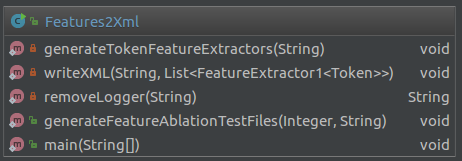
\includegraphics[scale=0.5]{gfx/Features2Xml.png}
\captionof{figure}{Class diagram of the Features2Xml class}
\label{fig:Features2Xml}


\section{Feature Ablation}
\label{sec:Ablation}
In this section the process of Feature Ablation that is done in this project gets described. The classes that are used for this are described in the section \ref{sec:Classes}. The goal of this process is to find the combination of Feature Extractors that yields the best NER results.

\subsection{General Approach}
\label{sec:AblationApproach}
To see the impact of the different Feature Extractors that are used during the NER, we evaluate the results of the NER when using different combinations of Feature extractors. Since only commenting out the extractors we want not to use in one single Ablation test and run the programm manually again and again, is very boring and takes a lot of time, we thought of an highly automated process which tests a lot of combinations of Feature Extractors. Theoretically we could test every single possible combination, which in our case would lead to $\sum_{k=1}^{n}\binom{n}{k} = 511$ different combinations, where $n = \left | M \right | = 9$ and $M = \{ FeatureExtractor_1, ..,  FeatureExtractor_n \}$ , denoting the set of Feature Extractors we us in the NER. We don't do this since firstly, it's not very useful to test all combinations since it is obvious that the results will be worse if only one or two Extractors are used and secondly, it would require too much computing power (i.e. time). One argument why one could do this anyways is, that one can get more detailed information about the impact of a single Feature Extractor on the result of the NER.\\
We think a good tradeoff would be if we test all possible combinations of Feature Extractors when using at least seven out of the nine Extractors we use in the NER. When doing this, the number of possible combinations gets reduced to $\sum_{k=7}^{9}\binom{9}{k} = 46$. Because this is still requires a lot of time to compute, we designed the algorithm to run the tests for the different combinations cuncurrently (see section \ref{sec:AblationTestRunner} and \ref{sec:ExecuteFeatureAblationTest} for more detailed information about the algorithm).\\
The algorithm is explained graphically in figure \ref{fig:AblationAlgo}

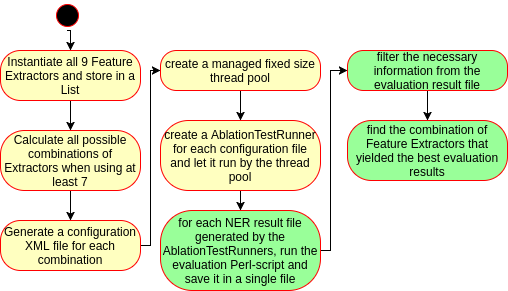
\includegraphics[scale=0.75]{gfx/ablationAlgo.png}
\captionof{figure}{(High level) Algorithm to find the best combination of Feature Extractors for NER}
\label{fig:AblationAlgo}


\subsection{Results}

\end{document}
